\section{MQTT - Instalación del controlador para ESP32}

Para comenzar con la implementación del sistema de monitoreo y control utilizando MQTT, se realizó la instalación de los controladores necesarios para el microcontrolador ESP32. La instalación se realizó siguiendo los pasos proporcionados en la guía del laboratorio y utilizando el Arduino IDE como entorno de desarrollo.

\subsection{Pasos de Instalación:}
\begin{enumerate}
    \item \textbf{Instalación de pyserial:}
    Se instaló la biblioteca \texttt{pyserial} debido a un requerimiento del sistema para habilitar la comunicación serial entre el entorno de desarrollo y el ESP32. Para ello, se utilizó el siguiente comando:
    \begin{lstlisting}[style=bashstyle]
    pip3 install --user --upgrade pyserial
    python3 -c "import serial, sys; print('pyserial -> OK', serial.__version__, sys.executable)"
    \end{lstlisting}
    
    \item \textbf{Carga de Código de Prueba en Arduino Uno:}
    Se cargó un código básico para comprobar la funcionalidad del ESP32, el cual hace parpadear el LED integrado del microcontrolador. Este paso es esencial para verificar que el entorno de desarrollo y el controlador estén correctamente configurados. El código cargado fue el siguiente:
    \begin{lstlisting}[style=cppstyle]
    void setup() {
      pinMode(LED_BUILTIN, OUTPUT);
    }
    void loop() {
      digitalWrite(LED_BUILTIN, HIGH); delay(500);
      digitalWrite(LED_BUILTIN, LOW); delay(500);
    }
    \end{lstlisting}
\end{enumerate}

\subsection{Problemas Encontrados y Soluciones:}
Durante la carga del código de prueba, surgieron problemas relacionados con la conexión del ESP32 al IDE de Arduino. Se solucionó ajustando las configuraciones del puerto COM y seleccionando correctamente la placa ESP32 en el menú de herramientas del IDE. Además, fue necesario poner el ESP32 en modo de carga manteniendo presionado el botón \texttt{BOOT} mientras se realizaba la carga.

Como se puede ver en la imagen \ref{fig:esp32_paso1}, el primer paso consistió en agregar la librería de ESP32 a los \texttt{board managers} de Arduino. En la imagen \ref{fig:esp32_paso2}, se muestra el proceso para instalar el Board de ESP32.

\begin{figure}[H]
    \centering
    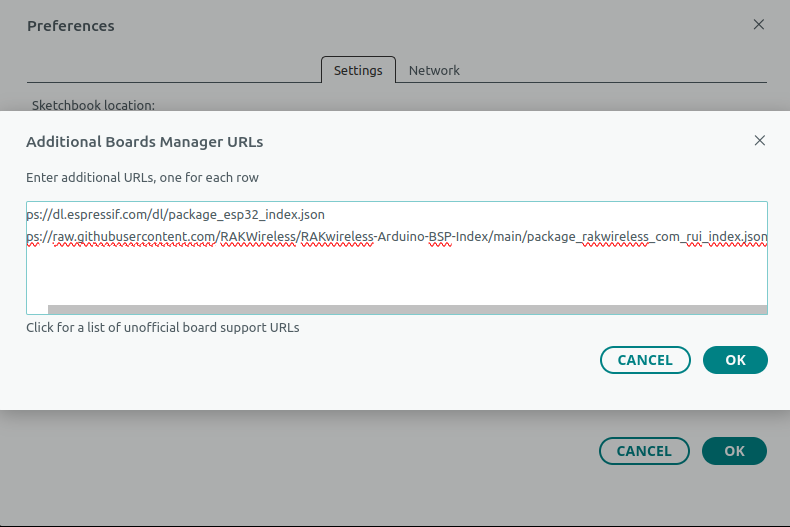
\includegraphics[width=0.85\textwidth]{./img/esp32_paso1.png}
    \caption{Agregando la librería de ESP32 a los board managers de Arduino Uno.}
    \label{fig:esp32_paso1}
\end{figure}

\begin{figure}[H]
    \centering
    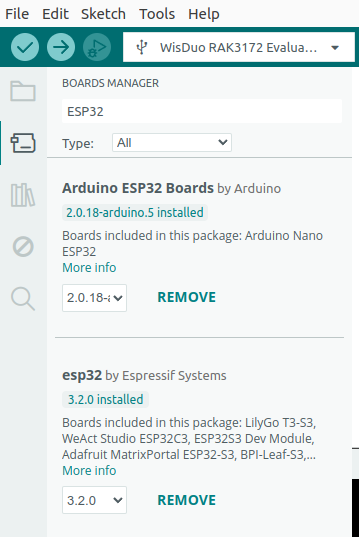
\includegraphics[width=0.85\textwidth]{./img/esp32_paso2.png}
    \caption{Instalación del Board de ESP32 en el Arduino IDE.}
    \label{fig:esp32_paso2}
\end{figure}

\section{MQTT - Implementación básica de sensor con ESP32}

Con el objetivo de implementar un sensor de temperatura (LM35) y humedad (DHT11) con el ESP32, se configuró un sistema que usa el protocolo MQTT para publicar y recibir datos.

\subsection{Comandos de Instalación:}
Se instaló el broker MQTT Mosquitto en la máquina local utilizando los siguientes comandos:
\begin{lstlisting}[style=bashstyle]
sudo apt-get update
sudo apt install mosquitto
sudo ufw allow 1883/tcp
sudo systemctl status mosquitto
sudo systemctl stop mosquitto
\end{lstlisting}

\subsection{Verificación de la Instalación:}
Se verificó la instalación del broker MQTT mediante los siguientes pasos:
\begin{itemize}
    \item Se levantó el broker con el comando:
    \begin{lstlisting}[style=bashstyle]
    sudo systemctl start mosquitto
    \end{lstlisting}
    \item Se verificó que estaba en funcionamiento mediante:
    \begin{lstlisting}[style=bashstyle]
    systemctl status mosquitto
    \end{lstlisting}
\end{itemize}

\subsection{Publicación y Recepción de Datos:}
El código de ESP32 para la publicación de datos de un sensor LDR fue el siguiente:
\begin{lstlisting}[style=cppstyle]
#define WIFI_SSID     "GalaxyS10+"
#define WIFI_PASSWORD "sksg2586"
#define MQTT_BROKER   "192.168.170.231"   // IP del PC con Mosquitto
#define MQTT_PORT     1883
#define MQTT_TOPIC    "iot/"

#include <WiFi.h>
#include <PubSubClient.h>

#define LDR_PIN 34        // GPIO del sensor LDR
const int ADC_MAX = 4095;  // resolucion de 12 bits (0-4095)

WiFiClient espClient;
PubSubClient mqtt(espClient);

void connectWiFi() {
  WiFi.begin(WIFI_SSID, WIFI_PASSWORD);
  while (WiFi.status() != WL_CONNECTED) {
    delay(500);
  }
}

void connectMQTT() {
  while (!mqtt.connected()) {
    if (mqtt.connect("ESP32_LDR_Client")) {
    } else {
      delay(2000);
    }
  }
}

void setup() {
  Serial.begin(115200);
  pinMode(LDR_PIN, INPUT);
  analogReadResolution(12);  // 12 bits = 0-4095
  connectWiFi();
  mqtt.setServer(MQTT_BROKER, MQTT_PORT);
  connectMQTT();
}

void loop() {
  if (WiFi.status() != WL_CONNECTED) connectWiFi();
  if (!mqtt.connected()) connectMQTT();
  mqtt.loop();

  int raw = analogRead(LDR_PIN);
  float light_norm = raw / (float)ADC_MAX;

  char payload[128];
  snprintf(payload, sizeof(payload), "{\"light_raw\": %u, \"light_norm\": %.3f}", raw, light_norm);

  mqtt.publish(MQTT_TOPIC, payload);
  delay(2000);
}
\end{lstlisting}

Como se puede ver en la imagen \ref{fig:mqtt_verify_install}, se verificó la instalación y ejecución del broker MQTT. En la imagen \ref{fig:mqtt_broker}, se muestra cómo se levanta el broker en la máquina local.

\begin{figure}[H]
    \centering
    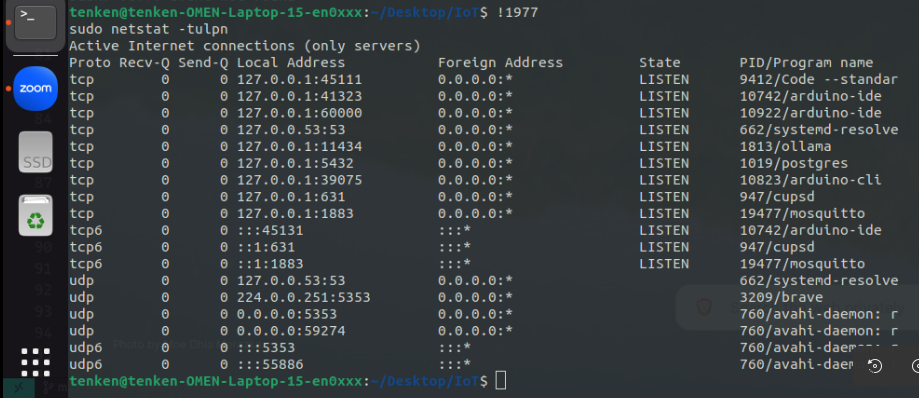
\includegraphics[width=0.85\textwidth]{./img/mqtt_verificar.png}
    \caption{Verificación de la instalación y ejecución del broker MQTT.}
    \label{fig:mqtt_verify_install}
\end{figure}

\begin{figure}[H]
    \centering
    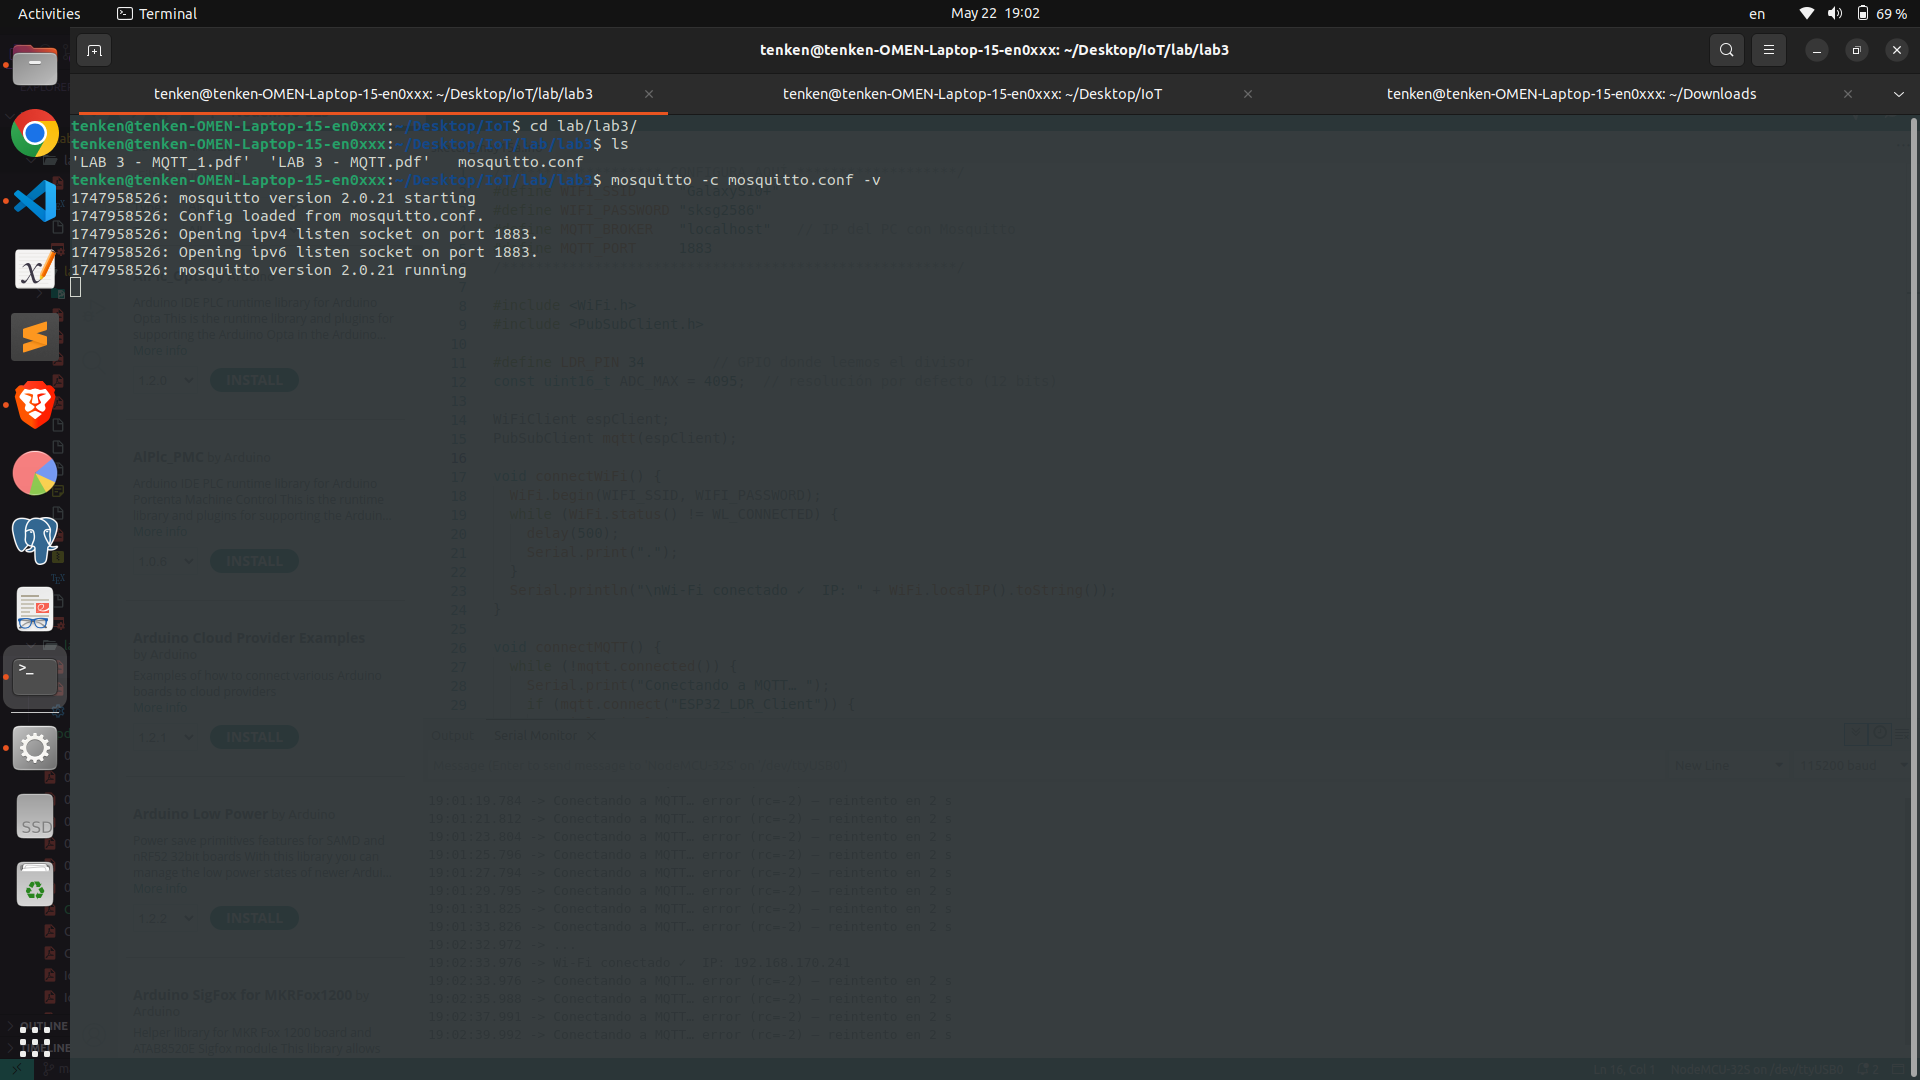
\includegraphics[width=0.85\textwidth]{./img/mqtt_conf_exec.png}
    \caption{Levantando el broker MQTT en la máquina local.}
    \label{fig:mqtt_broker}
\end{figure}

\begin{figure}[H]
    \centering
    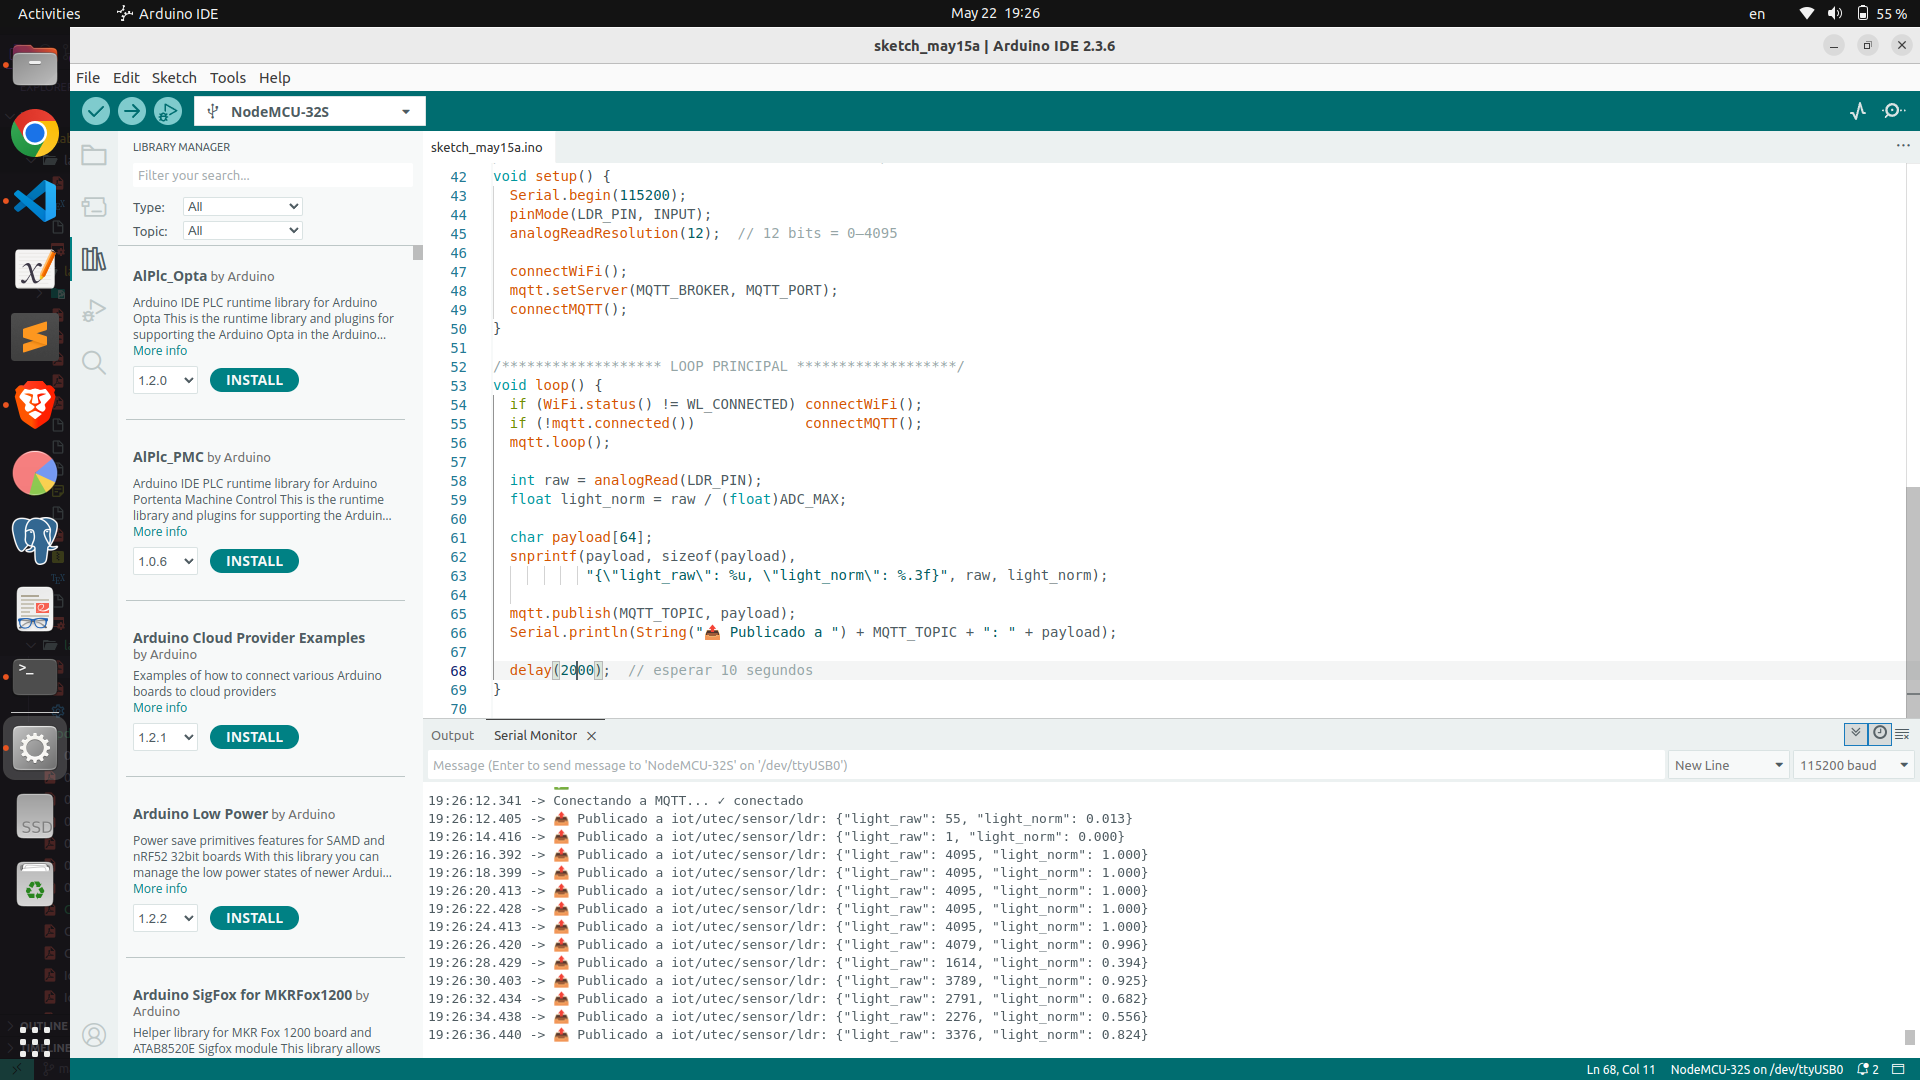
\includegraphics[width=0.85\textwidth]{./img/mqtt_publicando.png}
    \caption{Publicando los datos desde el sensor.}
    \label{fig:mqtt_publish}
\end{figure}

\begin{figure}[H]
    \centering
    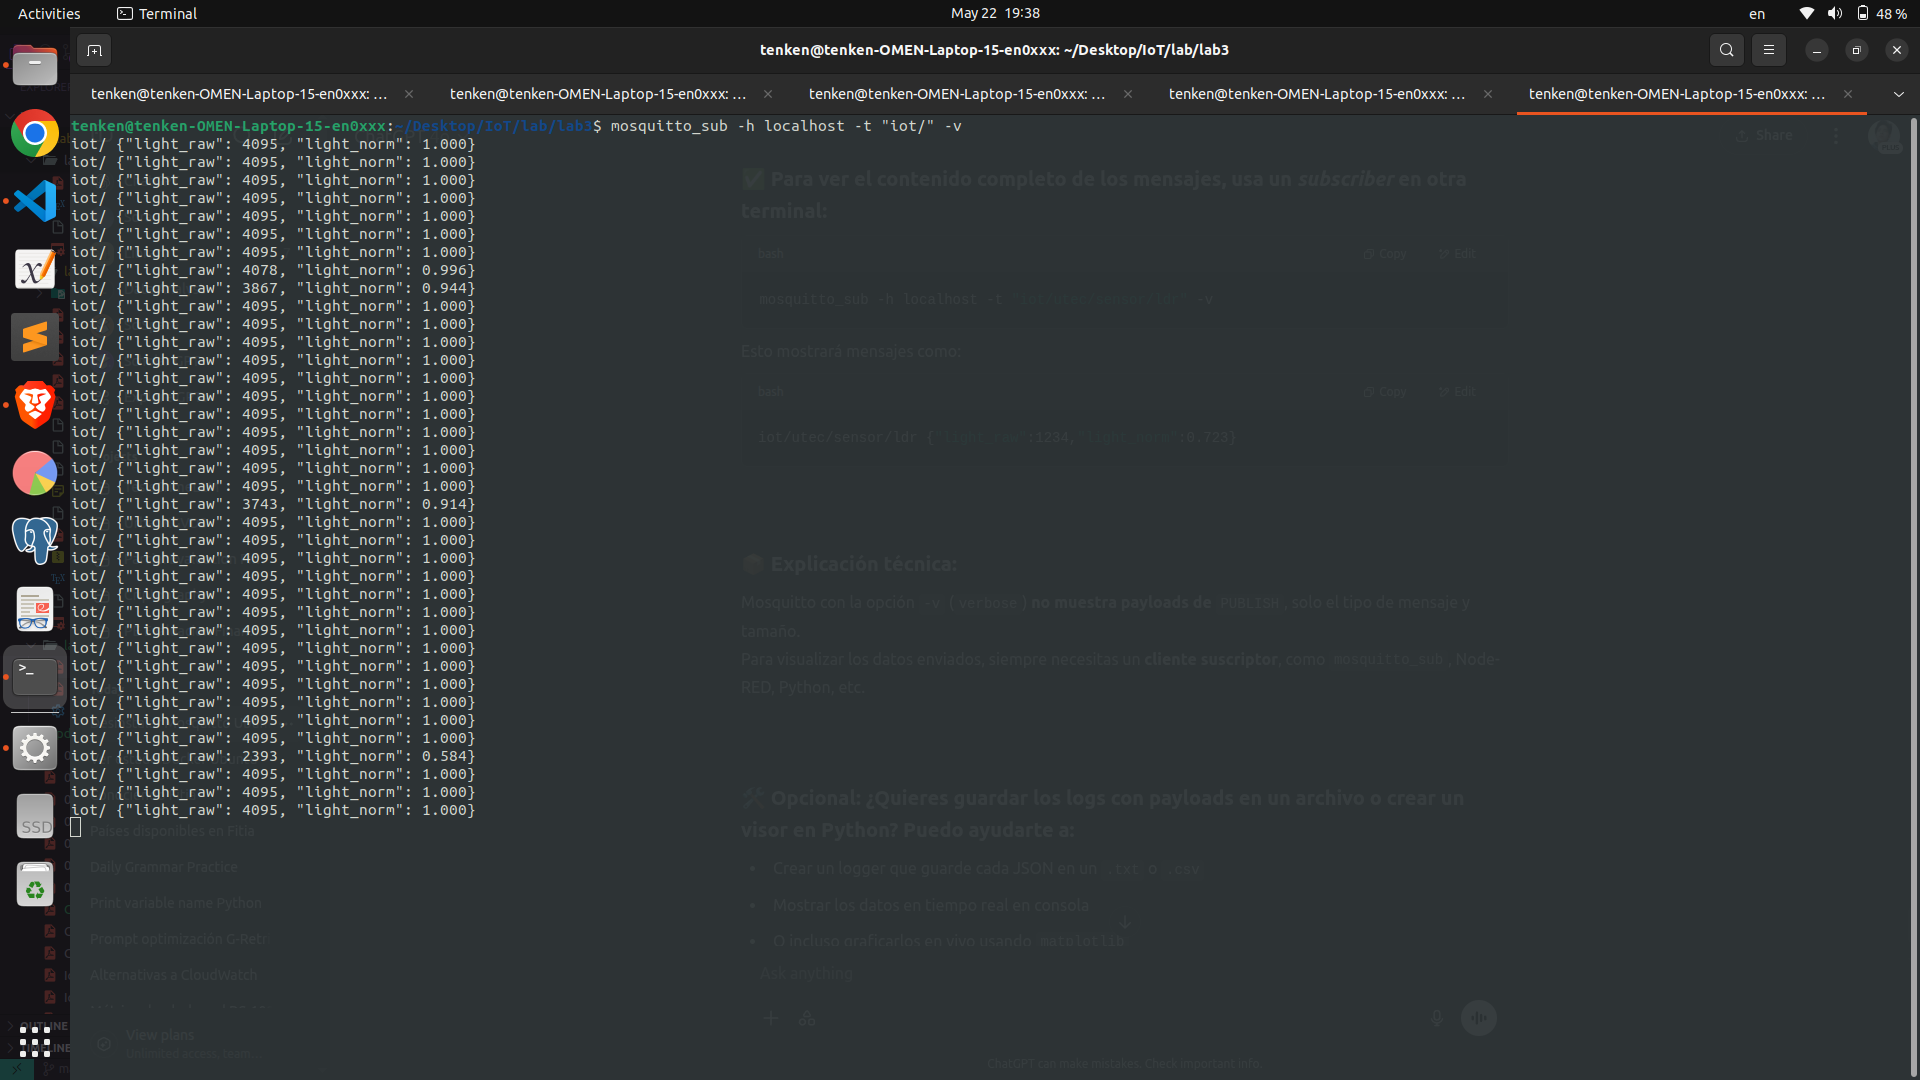
\includegraphics[width=0.85\textwidth]{./img/mqtt_suscribiendo.png}
    \caption{Recibiendo los datos desde el broker MQTT.}
    \label{fig:mqtt_subscribe}
\end{figure}
Finalmente, se comparte los diagramas de flujo \ref{fig:Diagrama_flujo_4_2} y diagramas de bloques \ref{fig:Diagrama_bloques_4_2} de la solucion implementada.
\begin{figure}[H]
    \centering
    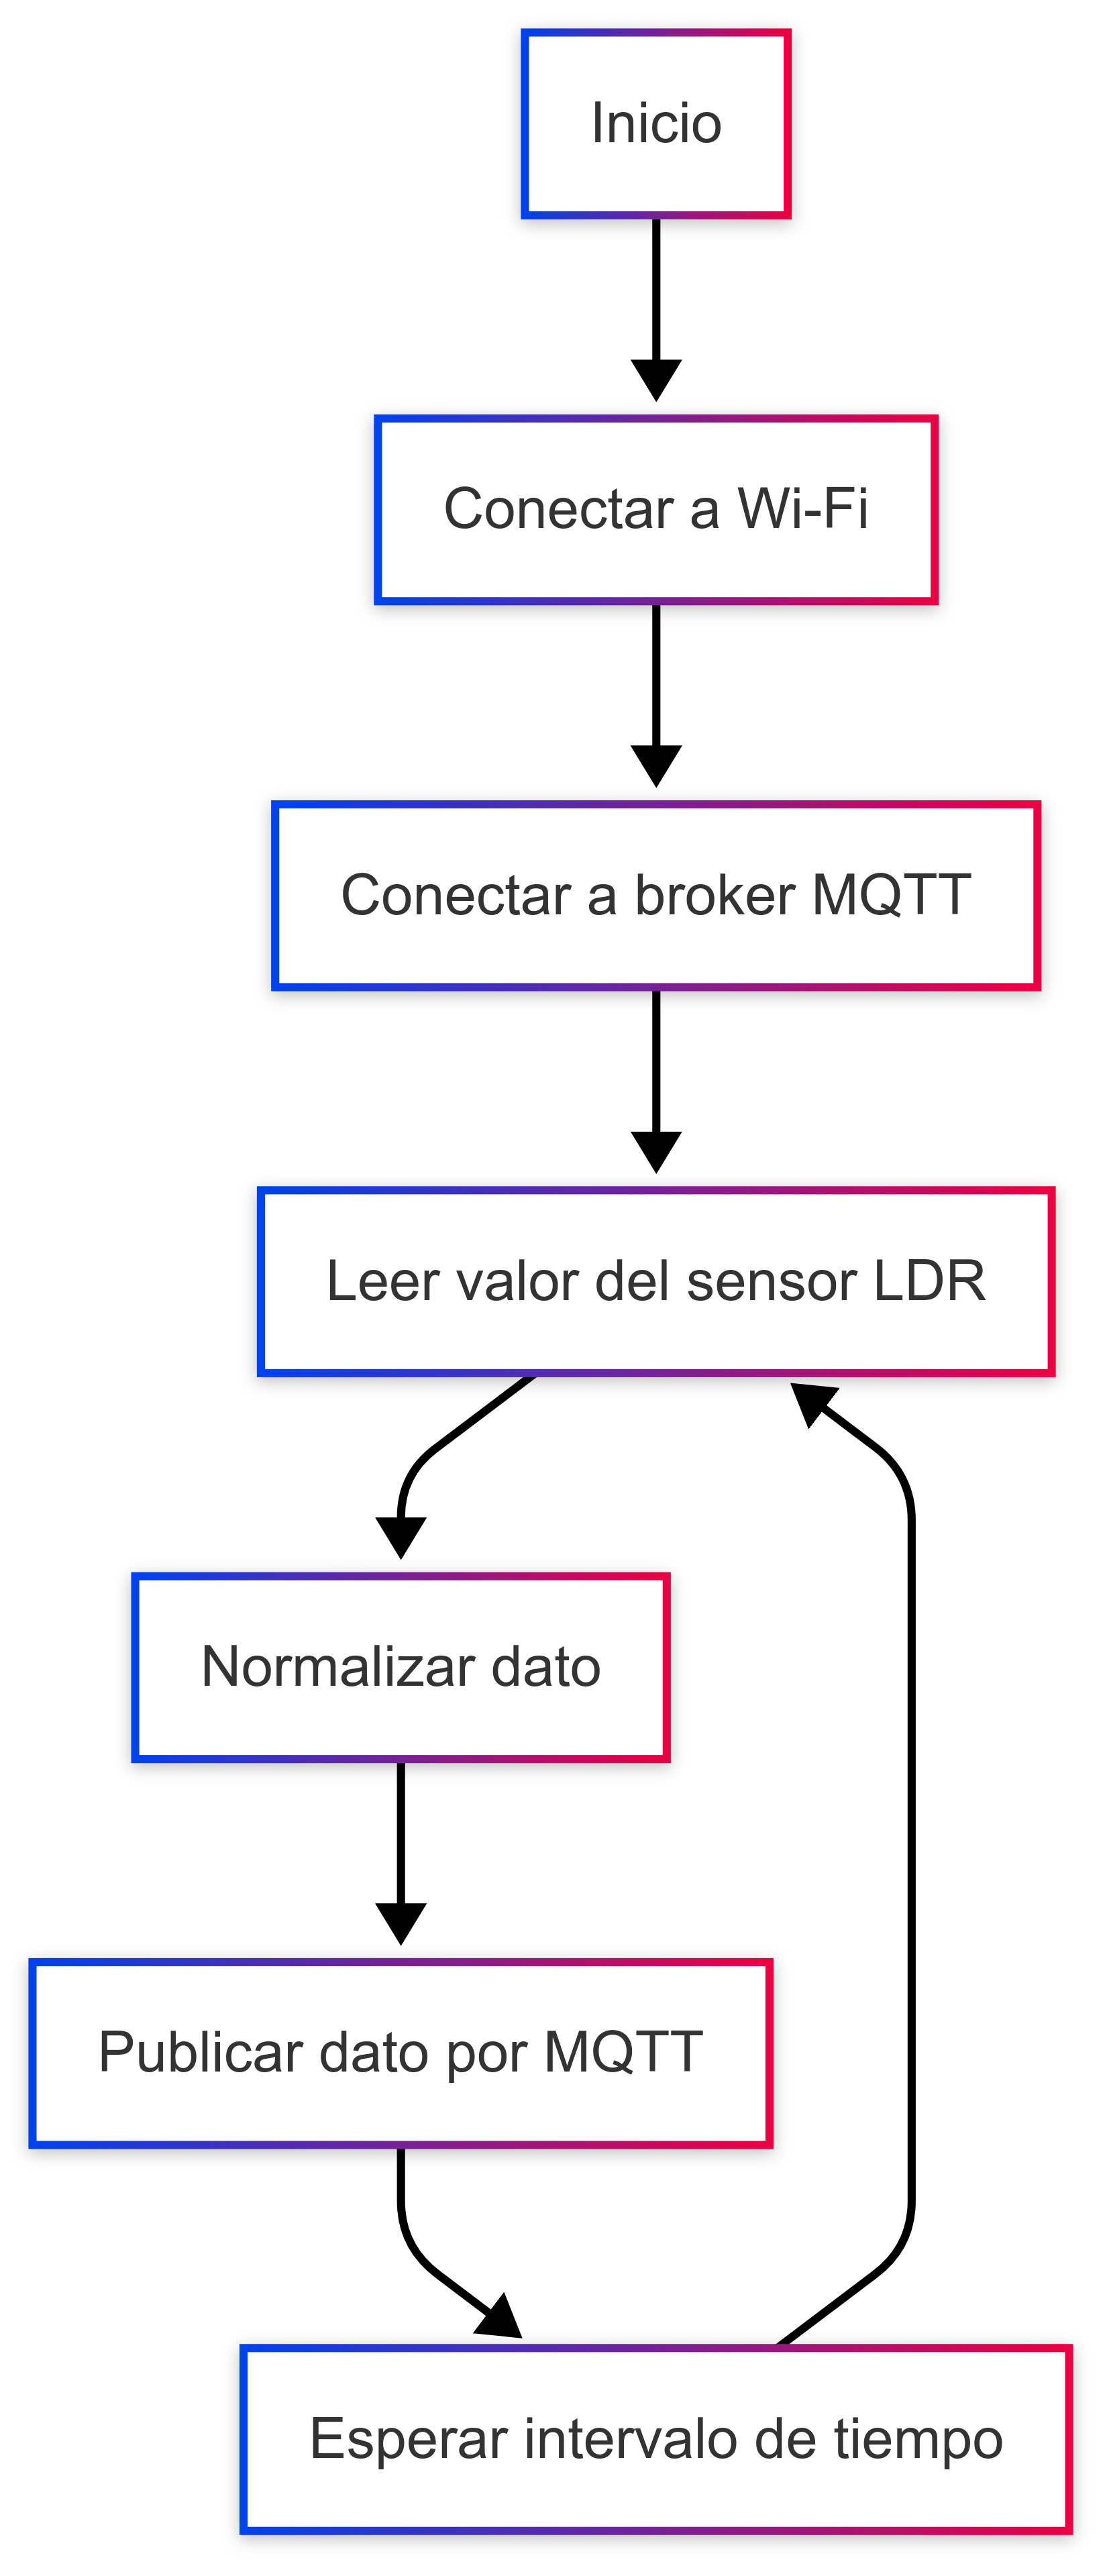
\includegraphics[width=0.3\textwidth]{./img/Diagrama_flujo_4_2.png}
    \caption{Diagrama de flujo de la solucion MQTT}
    \label{fig:Diagrama_flujo_4_2}
\end{figure}
\begin{figure}[H]
    \centering
    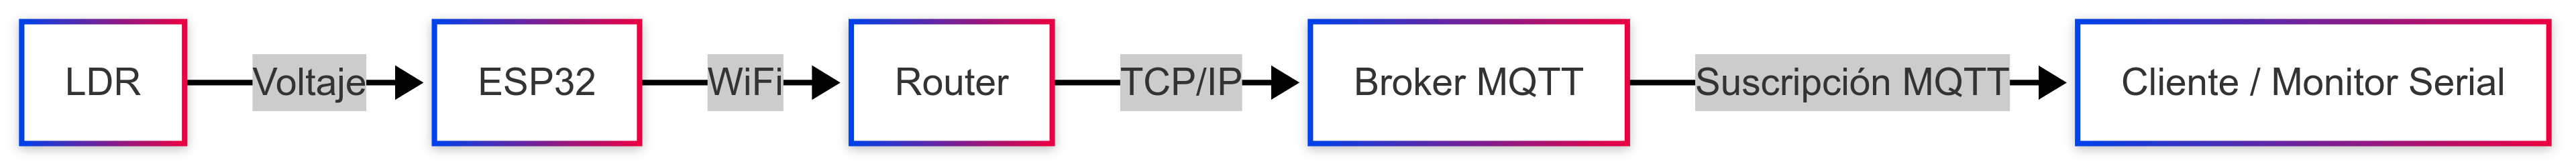
\includegraphics[width=0.85\textwidth]{./img/Diagrama_bloques_4_2.png}
    \caption{Diagrama de bloques de la solucion MQTT}
    \label{fig:Diagrama_bloques_4_2}
\end{figure}

\section{MQTT - Implementación con Sistema: Estación de Control Ambiental}

La siguiente fase fue integrar el sistema en una estación de control ambiental, que monitorea variables como la temperatura y la humedad. El sistema está basado en un Arduino Mega que se comunica con un ESP32 para transmitir los datos a través de MQTT a un broker Mosquitto.

\subsection{Componentes Utilizados:}
\begin{itemize}
    \item Arduino Mega
    \item ESP32
    \item Sensor LM35 (conectado a entrada analógica del Mega)
    \item Sensor DHT11 (conectado a entrada digital del Mega)
    \item Micro servo SG90
    \item Cables y protoboard
    \item LED Verde: ambiente normal
    \item LED Rojo: temperatura o humedad crítica
    \item LED Azul: modo de espera / carga
    \item Potenciómetro de 10k: conectado a entrada analógica A1 del Mega
\end{itemize}

\subsection{Lógica del Sistema:}
\begin{itemize}
    \item El Arduino Mega lee la temperatura desde el LM35 (conversión ADC).
    \item Lee la humedad relativa desde el DHT11.
    \item Si la temperatura > 30°C o la humedad > 70\%, el servo gira a 90° (simulando la apertura de un sistema de ventilación, compuerta o alarma mecánica).
    \item Si los valores vuelven a la normalidad, el servo regresa a 0°.
    \item El Mega envía los valores por UART (Serial) al ESP.
    \item El ESP los muestra por el monitor serial o los publica en una página web/local server o red WiFi interna.
\end{itemize}

\subsection{Resultados Esperados:}
\begin{itemize}
    \item El sistema debe responder en tiempo real a los cambios en los sensores, activando el servo cuando se superan los umbrales.
    \item Los datos deben ser visibles en el monitor serial del ESP32 y pueden ser accesibles desde otros dispositivos conectados al broker MQTT.
\end{itemize}

Como se puede observar en la imagen \ref{fig:estado_rojo}, el sistema muestra un estado rojo cuando se alcanza la temperatura o humedad crítica. En las imágenes \ref{fig:estado_verde} y \ref{fig:estado_azul}, se muestra el estado verde para condiciones normales y el estado azul para el modo de espera, respectivamente.

\begin{figure}[H]
    \centering
    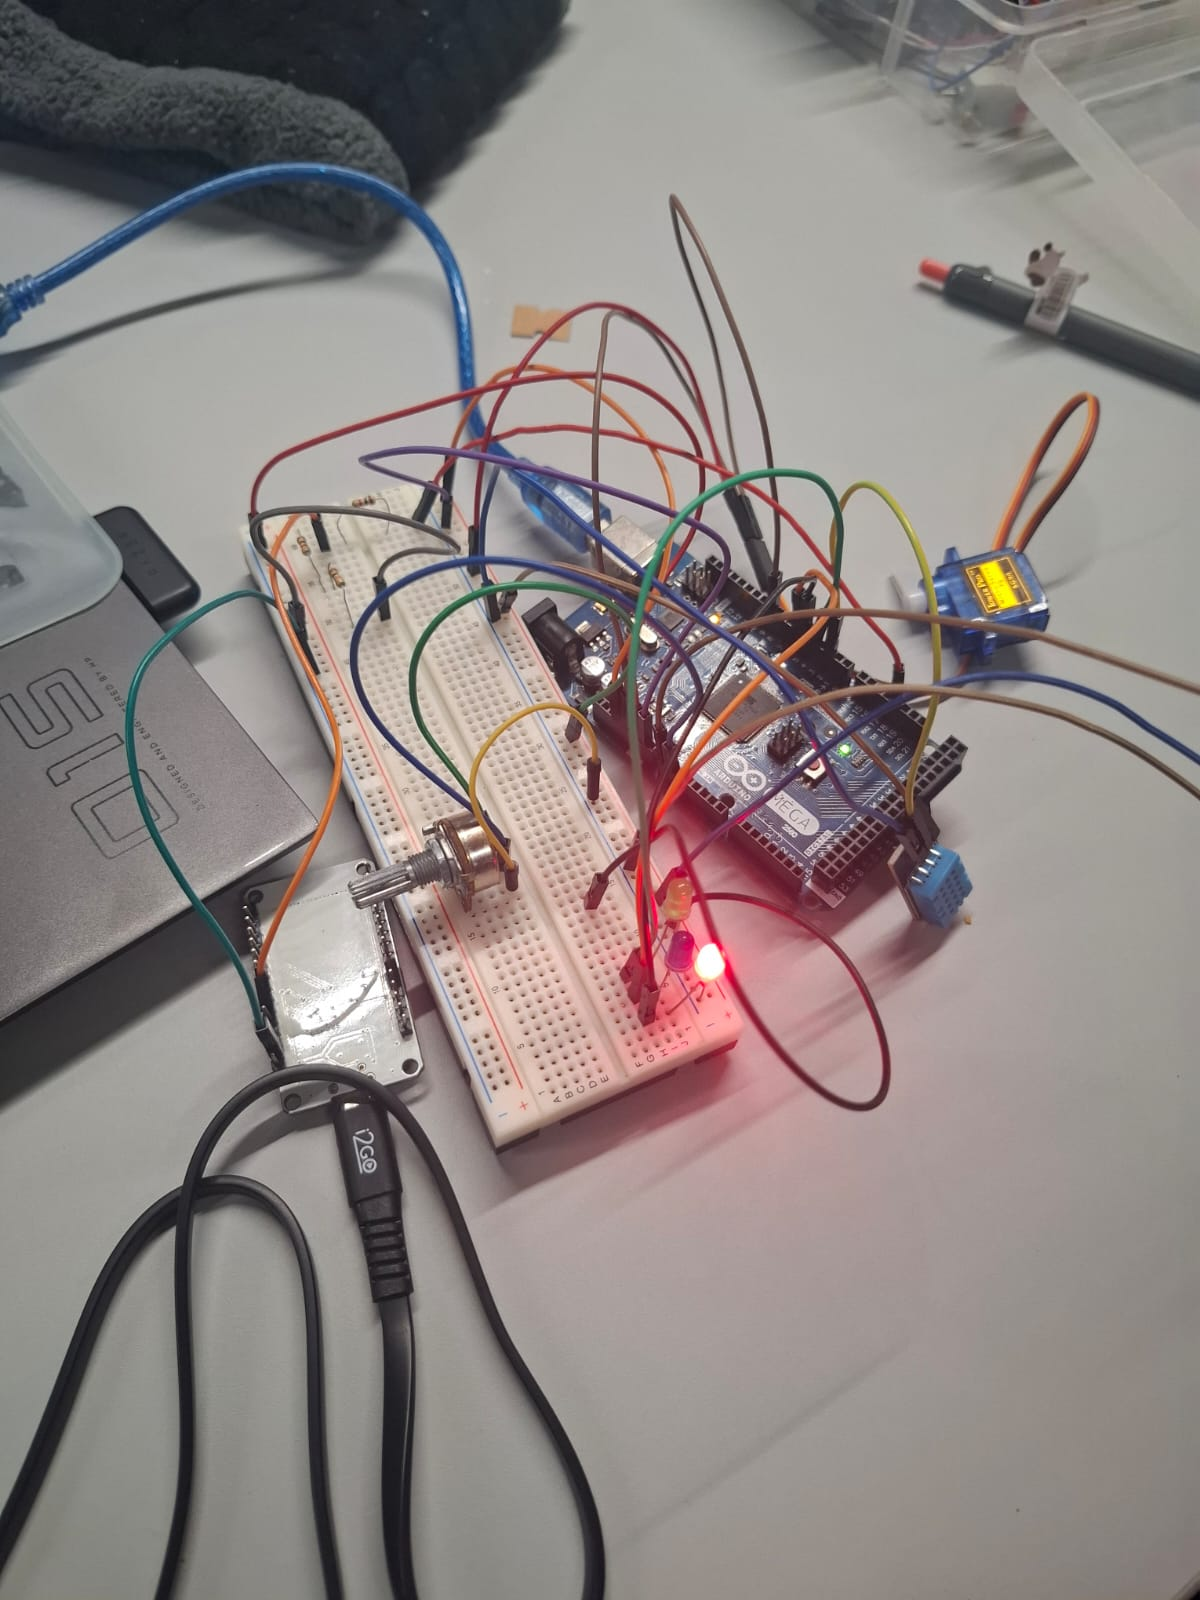
\includegraphics[width=0.85\textwidth]{./img/estado_rojo.jpeg}
    \caption{Estado rojo: Alerta de temperatura o humedad crítica.}
    \label{fig:estado_rojo}
\end{figure}

\begin{figure}[H]
    \centering
    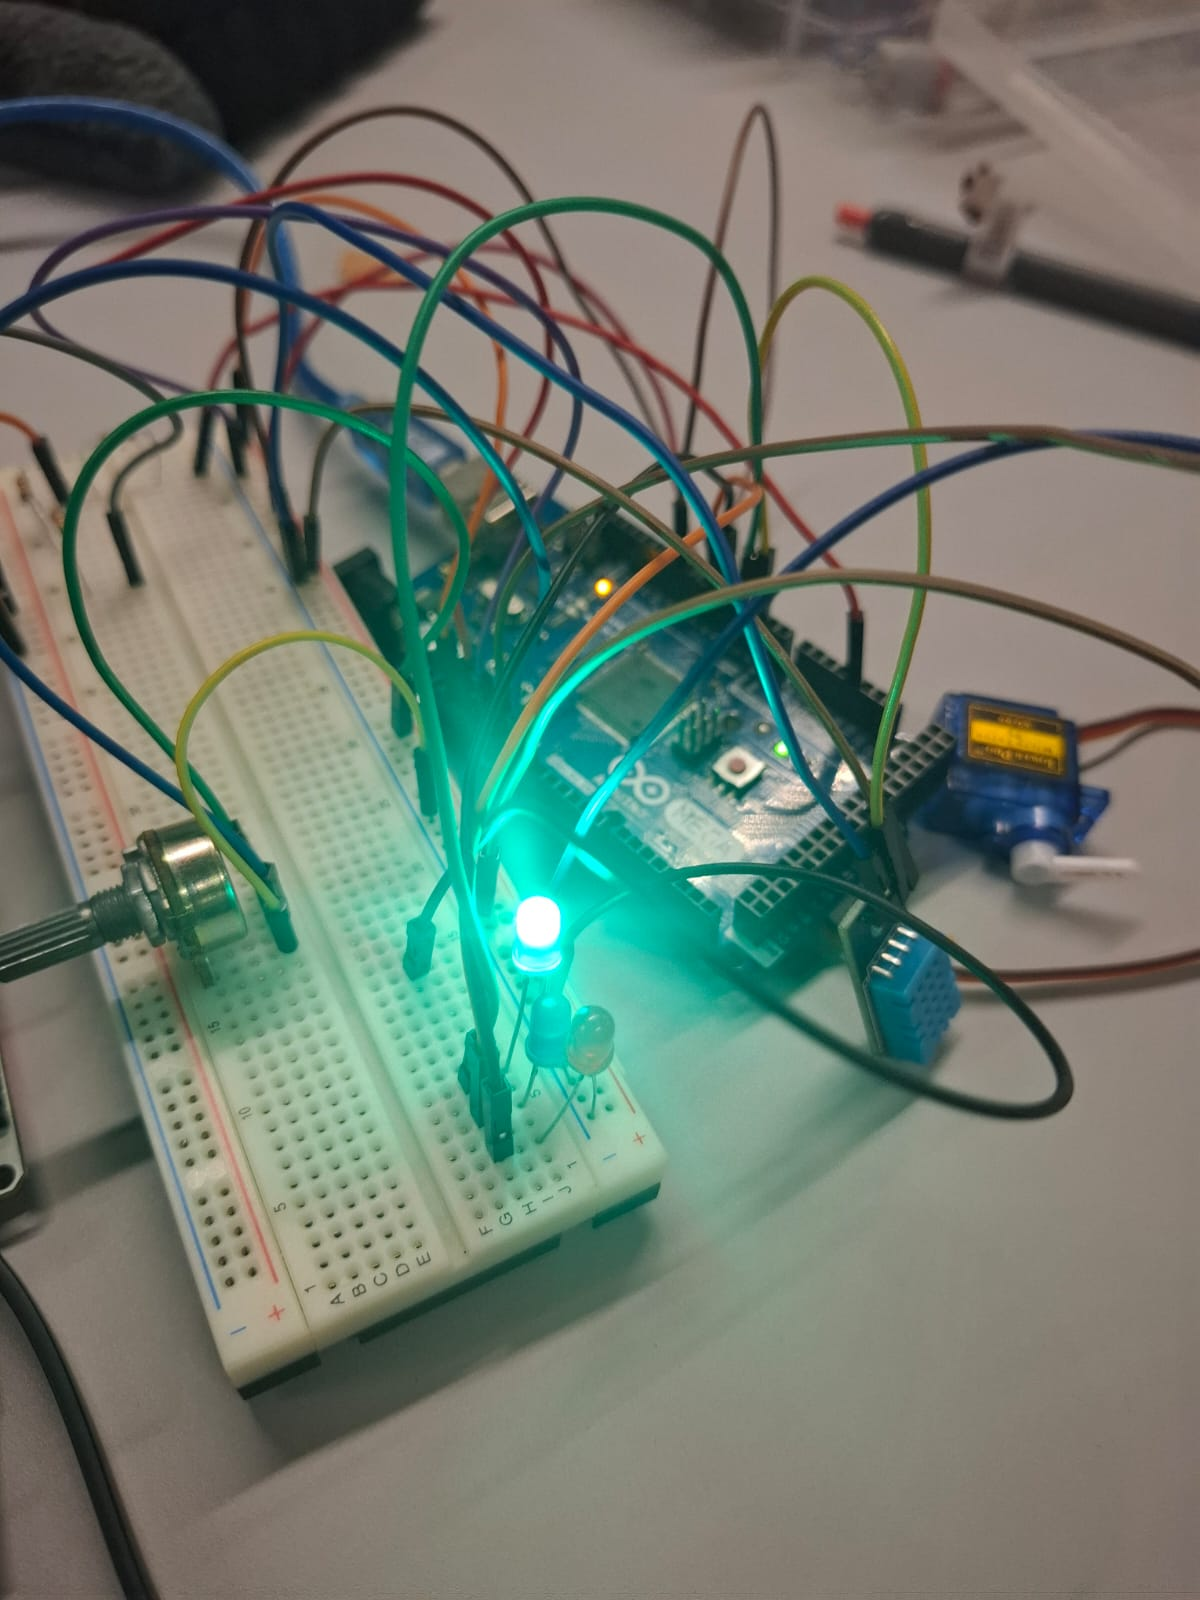
\includegraphics[width=0.3\textwidth]{./img/estado_verde.jpeg}
    \caption{Estado verde: Condiciones ambientales normales.}
    \label{fig:estado_verde}
\end{figure}

\begin{figure}[H]
    \centering
    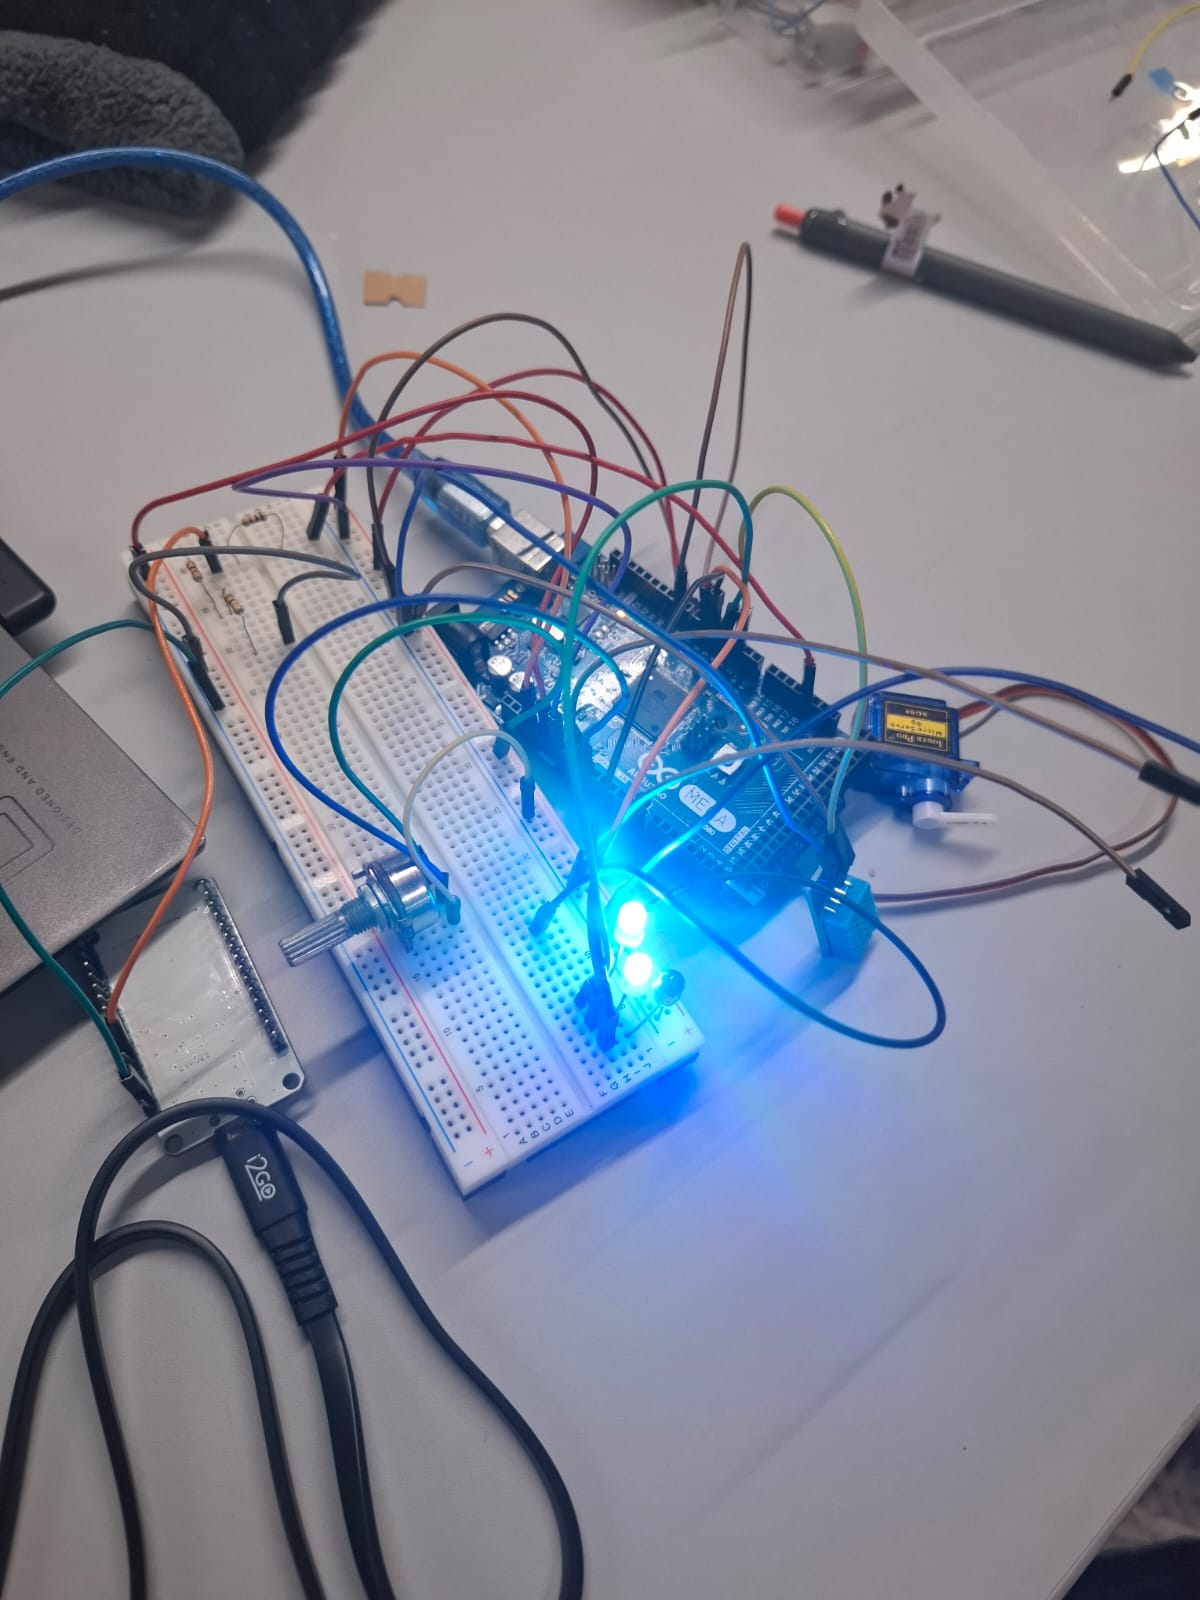
\includegraphics[width=0.85\textwidth]{./img/estado_azul.jpeg}
    \caption{Estado azul: Modo de espera / carga.}
    \label{fig:estado_azul}
\end{figure}

\begin{lstlisting}[style=cppstyle, caption={Código funcional de estación de control ambiental}, label={code:name}]
/******************************************************************
 * Estacion Ambiental - LM35 + DHT11 usando SimpleDHT
 * - Temperatura analogica (LM35)        -> A0
 * - Humedad digital    (DHT11)          -> D2
 * - Envio UART: "tempC_LM35,hum%\n"     -> ESP32 RX2 (9600 baud)
 ******************************************************************/
#include <SimpleDHT.h>

/* ---------- Pines ---------- */
#define LM35_PIN A0        // salida analogica del LM35
#define DHT_PIN  2         // pin DATA del DHT11 (10 k$/ohm$ pull-up a 5 V)

SimpleDHT11 dht11(DHT_PIN);

void setup() {
  Serial.begin(115200);     // Monitor serial
  Serial1.begin(9600);      // TX1 (pin 18) -> ESP32 RX2 (GPIO 16)
}

void loop() {
  /********** 1. Leer LM35 **********/
  int rawLM35 = analogRead(LM35_PIN);          // ADC 10-bit
  float tempC = rawLM35 * (5.0 / 1023.0) * 100.0;

  Serial.print("LM35 ADC: "); Serial.print(rawLM35);
  Serial.print(" -> Temp: "); Serial.print(tempC, 1); Serial.println(" C");

  /********** 2. Leer DHT11 **********/
  byte dhtTemp = 0, dhtHum = 0;
  int err = dht11.read(&dhtTemp, &dhtHum, NULL);

  if (err != SimpleDHTErrSuccess) {
    Serial.print("[WARN] Error leyendo DHT11: ");
    Serial.println(err);
    delay(2000);
    return;  // Saltar este ciclo si hay error
  }

  float humPct = (float)dhtHum; 

  Serial.print("Humedad: "); Serial.print(humPct, 0); Serial.println(" %");

  /********** 3. Enviar por UART **********/
  Serial1.print(tempC, 1);   Serial1.print(',');
  Serial1.print(humPct, 0); Serial1.print('\n');

  delay(2000);  // Tiempo minimo entre lecturas
}
\end{lstlisting}
Finalmente se adjuntan los diagramas de flujo y bloques para las solucion planteada para el control de ambiente.

\begin{figure}[H]
    \centering
    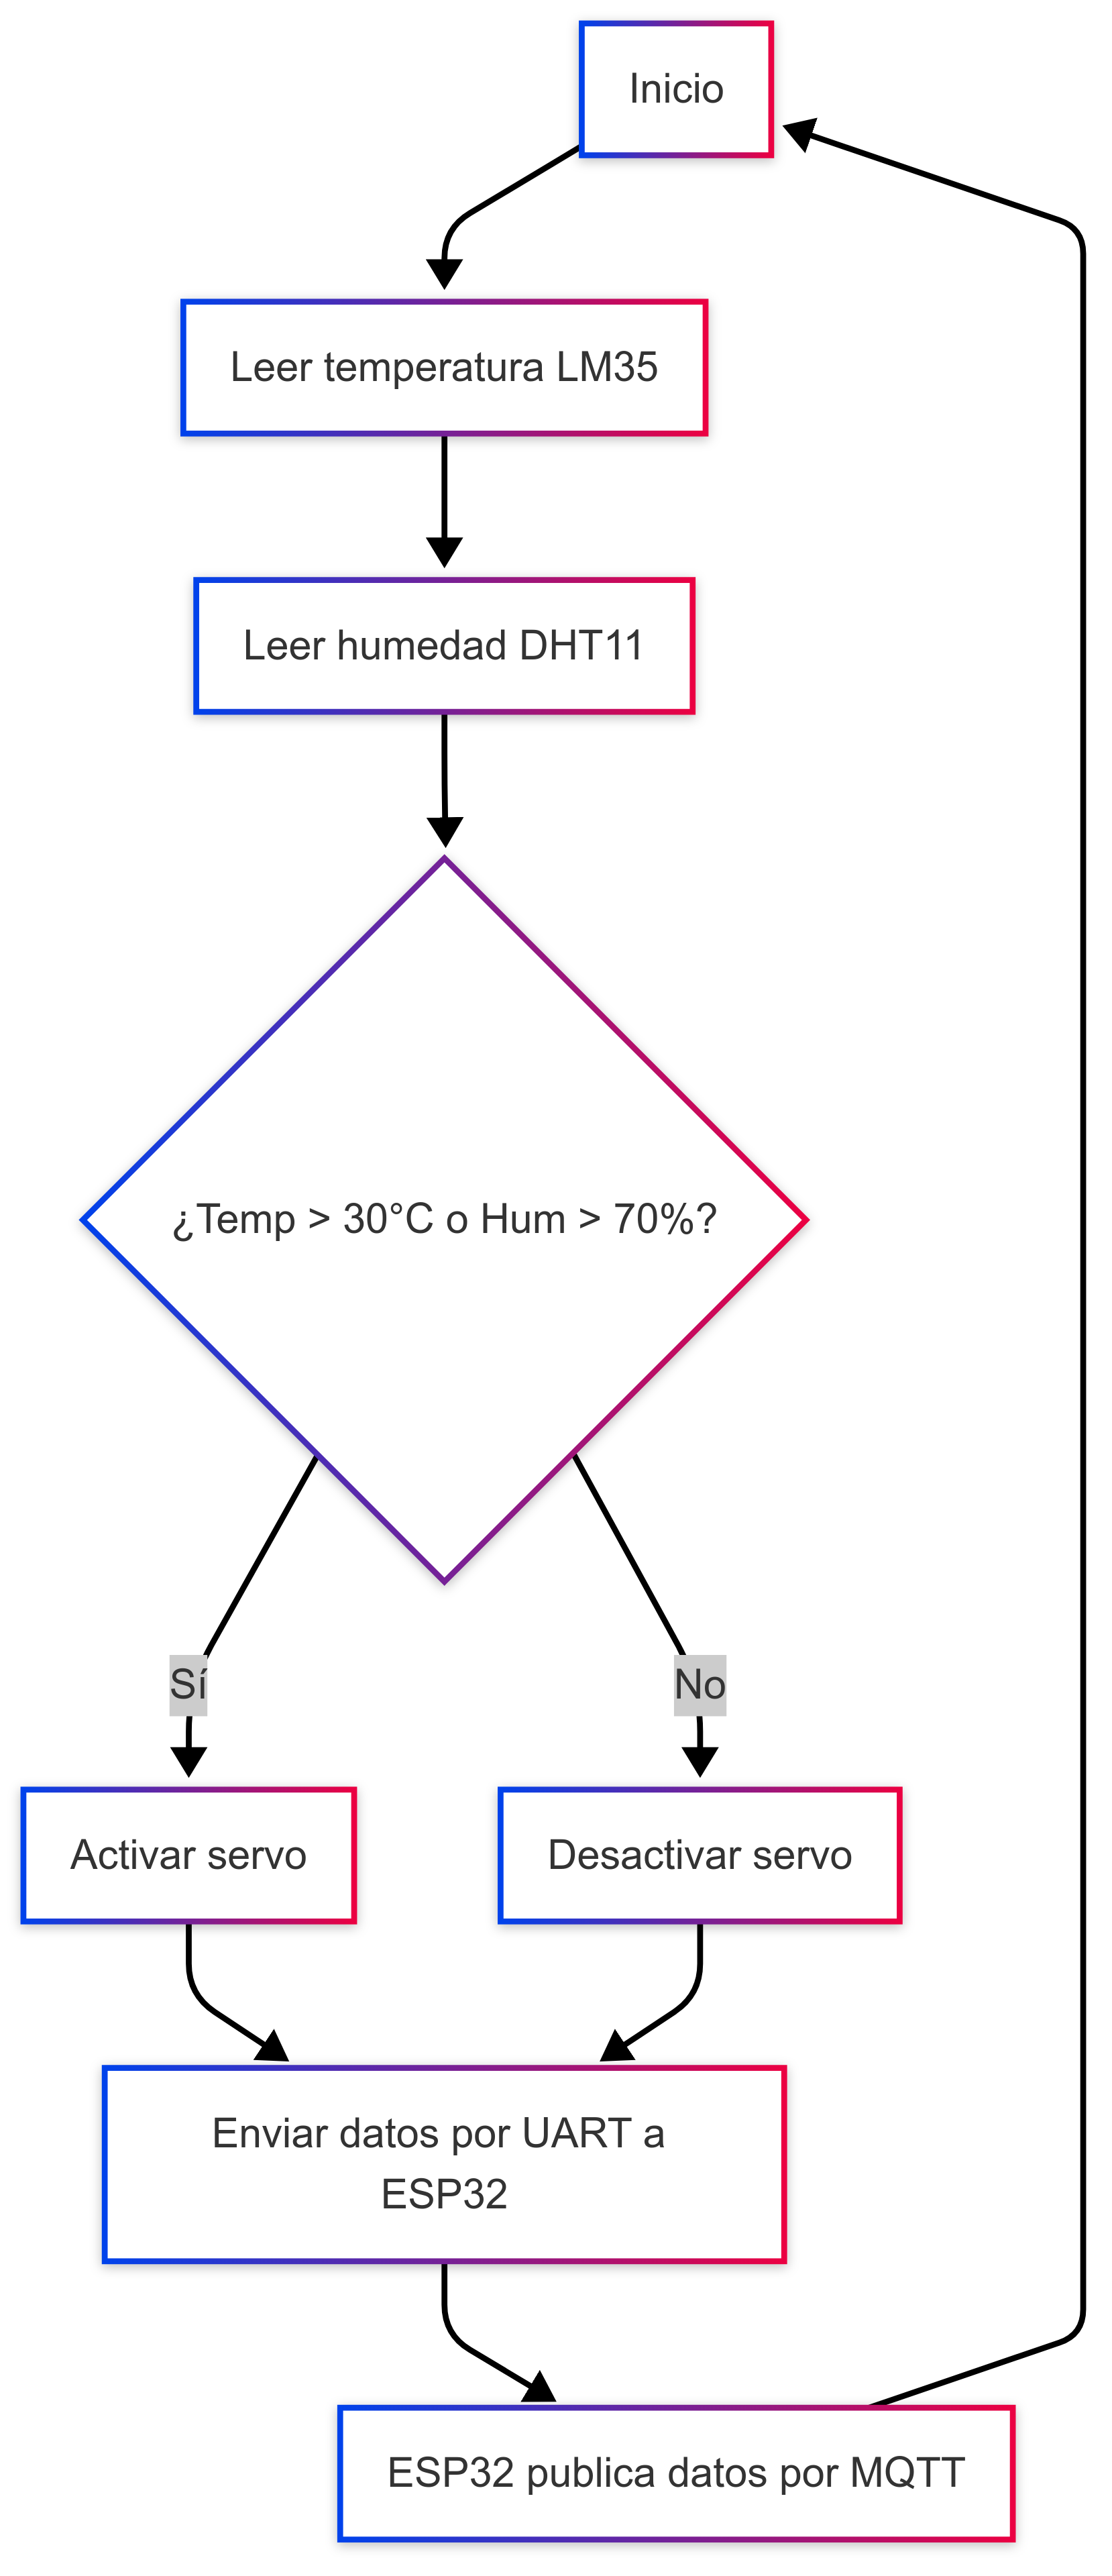
\includegraphics[width=0.85\textwidth]{./img/Diagrama_flujo_4_3.png}
    \caption{Diagrama de flujo para el control ambiental}
    \label{fig:Diagrama_flujo_4_3}
\end{figure}

\begin{figure}[H]
    \centering
    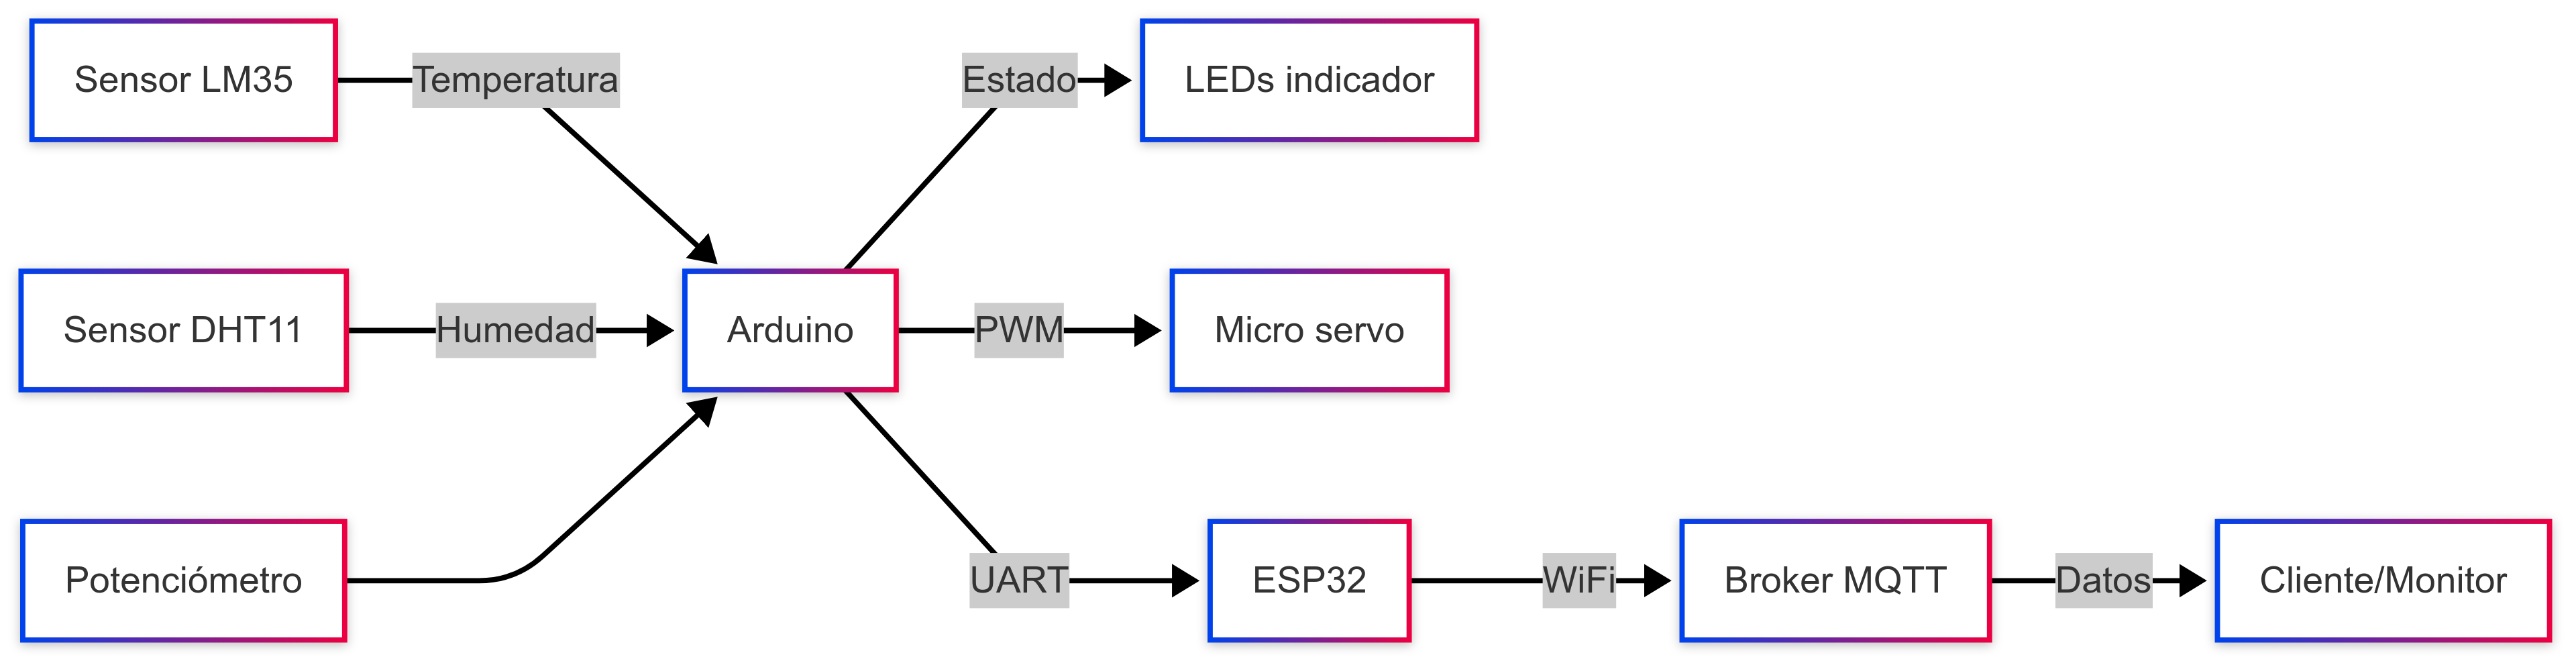
\includegraphics[width=0.85\textwidth]{./img/Diagrama_bloque_4_3.png}
    \caption{Diagrama de bloques para el control ambiental}
    \label{fig:Diagrama_bloque_4_3}
\end{figure}